\subsection{Instalación de git para Windows}
Para poder instalar git, nos vamos a dirigir a la página web de \textcolor{pucpRojo}{\href{https://git-scm.com/downloads}{git}}

\begin{figure}[!h]
	\centering
	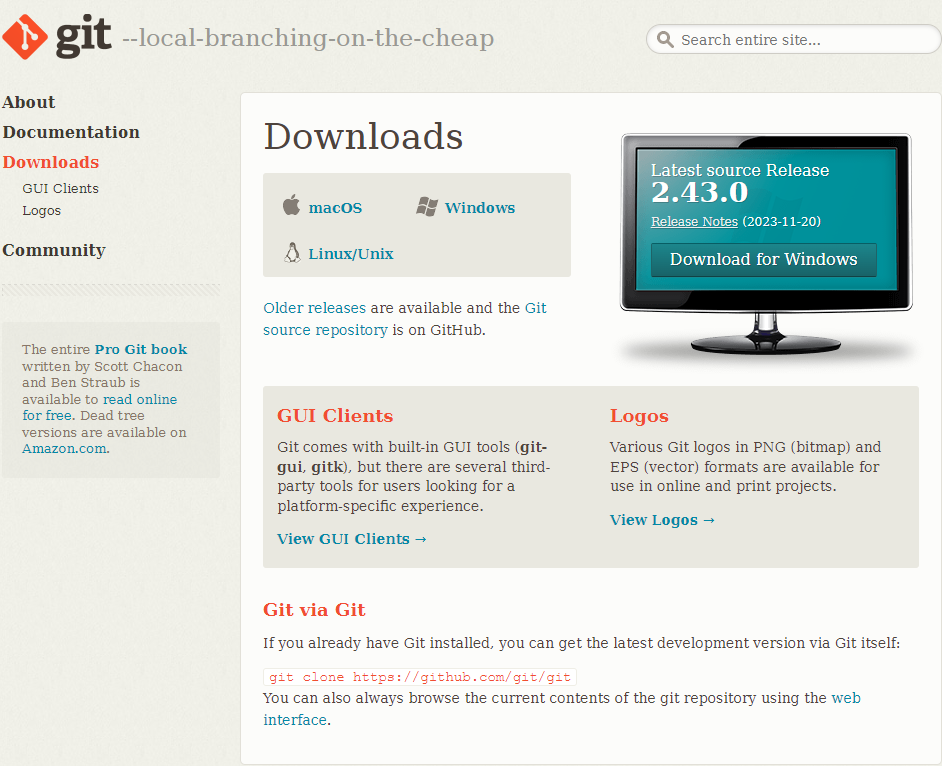
\includegraphics[width=0.50\textwidth]{01Instalacion/Imagenes/windows/instalacion01.png}
	\caption{Pagina de descarga de git}
	\label{fig:gitHomepage}
\end{figure}

Para nuestro caso vamos a descargar git según la versión de 32bits o 64 bits, según tenga nuestro computador.

\begin{figure}[!h]
	\centering
	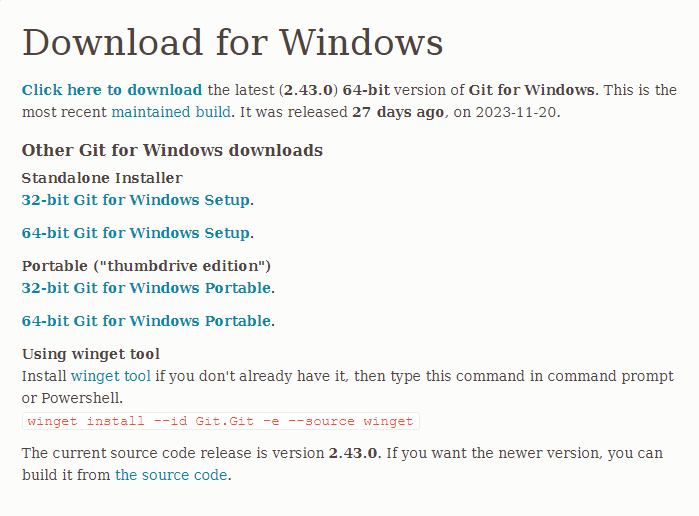
\includegraphics[width=0.50\textwidth]{01Instalacion/Imagenes/windows/instalacion02.png}
	\caption{Git: Instalación Windows}
	\label{fig:git}
\end{figure}

\newpage

Una vez termine al descargar, pasamos a ejecutarlo.

\begin{enumerate}
	\item Aceptamos la licencia GNU-GPL que tiene git.
	\begin{figure}[!h]
		\centering
		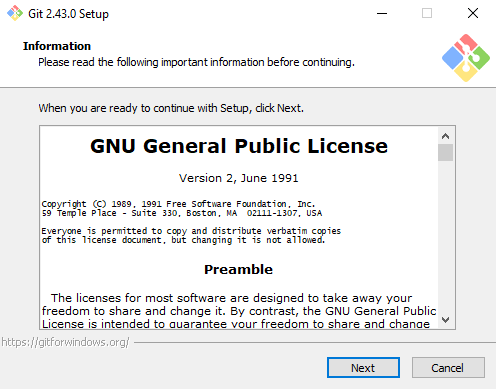
\includegraphics[width=0.5\textwidth]{01Instalacion/Imagenes/windows/instalacion03.png}
		\caption{Git: GNU General Public License}
		\label{fig:gitGPL}
	\end{figure}
	
	\item Escogemos la carpeta donde se desea que se instale Git, recomiendo dejarlo en su valor por defecto.
	\begin{figure}[!h]
		\centering
		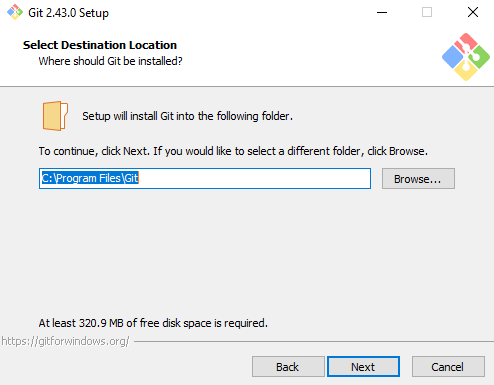
\includegraphics[width=0.5\textwidth]{01Instalacion/Imagenes/windows/instalacion04.png}
		\caption{Git: Carpeta de instalación}
		\label{fig:gitCaperta}
	\end{figure}
	\newpage
	\item Podemos cambiar la carpeta para los accesos directos del programa, pero de igual forma recomiendo dejarlo por defecto.
	\begin{figure}[!h]
		\centering
		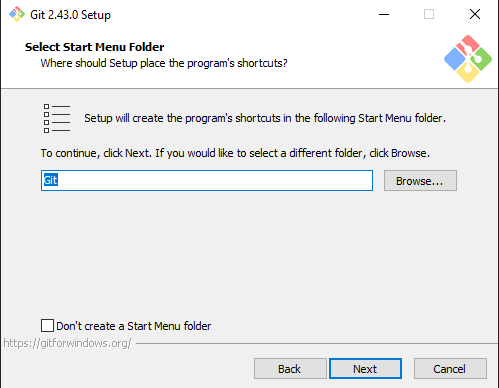
\includegraphics[width=0.5\textwidth]{01Instalacion/Imagenes//windows/instalacion06.png}
		\caption{Git: Carpeta de acceso directo}
		\label{fig:gitAccesoDirecto}
	\end{figure}
	
	\item Ahora en git, cuando vayamos a realizar un \emph{commit} o alguna configuración desde la terminal, vamos a necesitar de un editor de texto, por defecto este viene con \emph{Vim}. Recomiendo escoger el que le sea más comodo, en caso no este familiarizado con las keybindings de \emph{Vim}.
	\begin{figure}[!h]
		\centering
		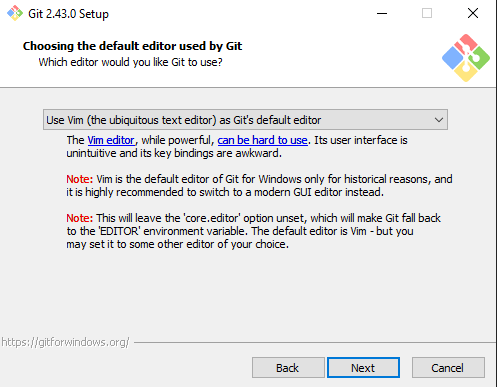
\includegraphics[width=0.5\textwidth]{01Instalacion/Imagenes/windows/instalacion07.png}
		\caption{Git: Editor por defecto }
		\label{fig:gitEditor}
	\end{figure}
	\newpage
	\item Por defecto se va a estar marcada la opción de \textbf{Let Git decide}. Esto porque historicamente cuando creemos un nuevo repositorio con git(esto se vera más adelante) la rama principal se suele crear con el nombre de \emph{Master}, pero como nosotros vamos a estar trabajando adicionalmente con \textit{Github}, este recomienda que el nombre de la rama principal se denomine como \emph{main}. De igual forma, más adelante veremos como podemos cambiarle el nombre a la rama principal.
	\begin{figure}[!h]
		\centering
		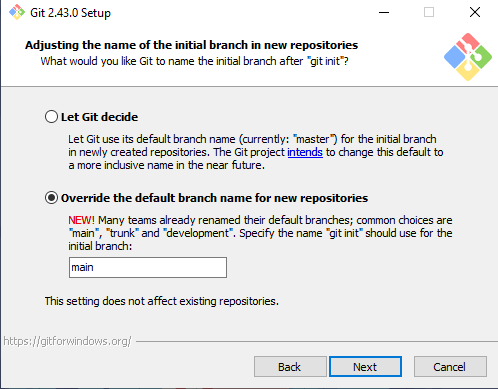
\includegraphics[width=0.5\textwidth]{01Instalacion/Imagenes/windows/instalacion08.png}
		\caption{Git: Rama principal}
		\label{fig:gitMainBranch}
	\end{figure}
	
	\item Recomiendo dejar los ajuste del PATH por defecto, pero de igual manera los puede modificar según sus necesidades
	\begin{figure}[!h]
		\centering
		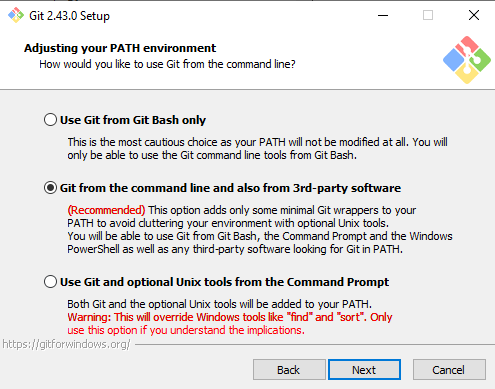
\includegraphics[width=0.5\textwidth]{01Instalacion/Imagenes/windows/instalacion09.png}
		\caption{Git: Ajuste del PATH}
		\label{fig:gitPATH}
	\end{figure}
	\newpage
	\item Todas las demás opciones que siguen, recomiendo dejarlo por defecto.
	\item Con esto ya terminamos de instalar git, y si buscamos dentro de nuestro programas vamos a poder verificar su instalación.
	\begin{figure}[!h]
		\centering
		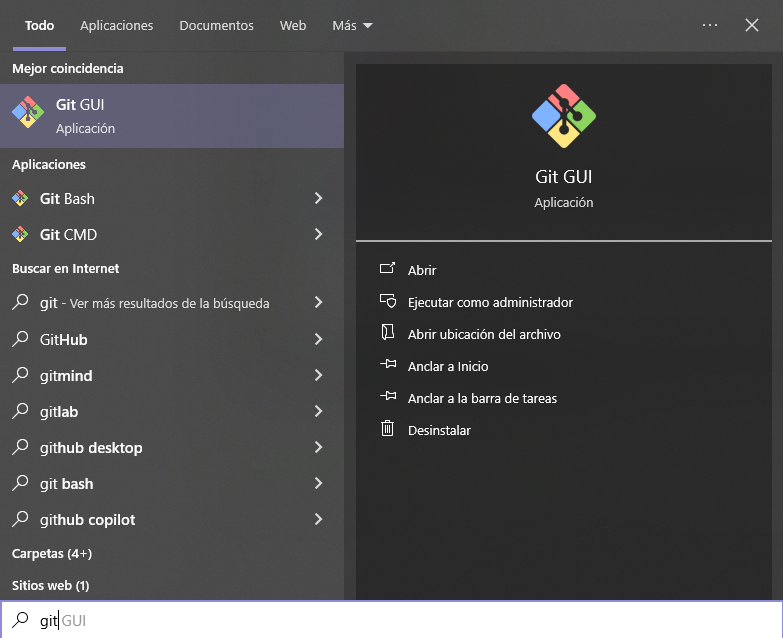
\includegraphics[width=0.5\textwidth]{01Instalacion/Imagenes/windows/instalacion10.png}
		\caption{Git: Verificación de instalación}
		\label{fig:gitInstaladoWindows}
	\end{figure}
\end{enumerate}